\documentclass[ppgc,espec]{iiufrgs}
\usepackage[utf8]{inputenc}   % pacote para acentuação
\usepackage{graphicx}           % pacote para importar figuras
%\usepackage{times}              % pacote para usar fonte Adobe Times
\usepackage[alf,abnt-emphasize=bf]{abntex2cite}	% pacote para usar citações abnt
\usepackage{multirow}

\title{Normas para Apresentação de Monografias do Instituto de Informática}
\espec{Engenharia de Software}
\author{Aluno}{Nome do}
\advisor[Profa.~Dra.]{Aluno}{Nome do(a) Orientador(a) do}
\date{mes}{2017}   % a data deve ser a da defesa
\location{Porto Alegre}{RS}
\keyword{ABNT}
\keyword{processadores de texto}
\keyword{formatação eletrônica de documentos}


% inicio do documento
\begin{document}
\maketitle
\chapter*{Agradecimentos}

Quando desejado pelo autor do trabalho, são apresentados logo após a folha de rosto, nessa ordem. São de livre apresentação gráfica. Geralmente os Agradecimentos são apresentados como um capítulo não-numerado. O mesmo é recomendado para os próximos itens, até o Resumo e Abstract.

\tableofcontents
% o parametro deve ser a abreviatura mais longa
\begin{listofabbrv}{UFRGS}
    \item[BB] Banco do Brasil
    \item[CC] Código Civil
    \item[BR] Brasil
    \item[UFRGS] Universidade Federal do Rio Grande do Sul
    \item[BD] Banco de Dados
\end{listofabbrv}

\listoffigures
\listoftables
\begin{abstract}

Consiste na apresentação clara e concisa dos pontos relevantes do trabalho, de maneira a permitir ao leitor saber da conveniência ou não da sua leitura na íntegra. É redigido pelo autor, em português e em inglês, em páginas distintas, antecedendo a introdução. Cada um ocupará no máximo 1 folha, e poderão ter \emph{até 500 palavras}. Para maiores informações com relação à redação consultar a NBR-6028 da ABNT (1990).

Quanto ao estilo, o resumo deve ser composto por uma seqüência de frases completas e não por uma enumeração de tópicos; a primeira frase deverá ser significativa, explicando o tema principal do documento. Na redação, dar preferência ao uso da terceira pessoa do singular e do verbo na voz ativa. Após o resumo e o abstract devem constar palavras-chave relativas aos assuntos da monografia, em português e inglês respectivamente. Estas são alinhadas na margem inferior do documento.

A ABNT define resumo como: ``[\ldots] seqüência de frases concisas e objetivas e não de uma simples enumeração de tópicos, não ultrapassando 500 palavras, seguido logo abaixo, das palavras representativas do conteúdo do trabalho, isto é, palavras-chave e/ou descritores, conforme a NBR 6028.''

Este item serve para informar o conteúdo do trabalho, orientando assim, o leitor na certeza da continuidade, ou desistência  da leitura do mesmo.
\end{abstract}

\begin{englishabstract}{This should be the title in English}{ABNT, text processors, electronic document preparation}

This work has the purpose of\ldots

O abstract deve apresentar, adicionalmente, uma tradução do título do trabalho. O título traduzido é colocado antes do título do capítulo (``Abstract''), a 2cm da margem superior, centralizado, em fonte Times 14 pt negrito.

Ocupará no máximo 1 folha, e poderão ter \emph{até 500 palavras}. Para maiores informações com relação à redação consultar a NBR-6028 da ABNT (1990).

Trabalhos de conclusão de especialização normalmente \emph{não exigem} a inclusão de Abstract em inglês.
\end{englishabstract}

\chapter{Orientações gerais}

Este capítulo tem o objetivo de descrever os detalhes necessários à correta formatação do documento. As informações aqui apresentadas devem ser suficientes para formatar corretamente o documento com qualquer ferramenta de edição.

Este documento foi criado utilizando estilos. Observe isso com atenção.

Os capítulos são sempre iniciados em uma nova folha. O título do capítulo é formatado todo em letras maiúsculas, com fonte Helvetica (ou semelhante) tamanho 16 pt, em negrito. Para os capítulos não-numerados (Listas, Resumo, Abstract, Referências, etc.), o título é centralizado na linha. Para os numerados, é alinhado à esquerda, precedido do respectivo número. Deve-se deixar 90 pt de espaçamento anterior (ou seja, distância da margem superior) e 42 pt de espaçamento posterior (espaço até o início do texto ou primeira subdivisão). O texto deve ser escrito em espaçamento simples, com observância de 6 pt de espaçamento em relação ao parágrafo seguinte.

\section{Sobre os títulos e capítulos}

As demais subdivisões do texto (seções, subseções, etc.) são formatadas com o título alinhado sempre à esquerda, precedido da respectiva numeração. Esta é formada pela união dos números relativos a cada nível de subdivisão, separados por pontos. Não se inclui um ponto no final.

São permitidas subdivisões até o 5º. nível (onde o capítulo é o 1º. nível), porém no sumário inclui-se somente os títulos até o nível 3. Os parâmetros para formatação dos títulos e espaçamentos nos diversos níveis de subdivisões são apresentados na Tabela \ref{tab:formatacao-subdivisao}.

\begin{table}[h]
    \caption{Parâmetros para formatação das subdivisões do texto}
    \begin{center}
        \begin{tabular}{ c | c | c | c | c }
            \hline
            Nível & Tamanho & Estilo & Esp. Antes & Esp. Depois \\
            \hline
            1 (capítulo) & 16 pt & negrito, maiúsc. & 90 pt & 42 pt \\
            \hline
            2 (seção) & 14 pt & negrito & 18 pt & 9 pt \\
            \hline
            3 (subseção) & 12 pt & negrito & 12 pt & 6 pt \\
            \hline
            4 & 12 pt & itálico & 12 pt & 6 pt \\
            \hline
            5 & 12 pt & normal & 12 pt & 6 pt \\
            \hline
        \end{tabular}
    \end{center}
    \legend{Fonte: \citeauthor{furaste2000}, \citeyear{furaste2000}, p. 49-56.}
    \label{tab:formatacao-subdivisao}
\end{table}

\subsection{Sobre o sumário}

Relaciona as principais divisões e seções do texto, na mesma ordem em que nele se sucedem, indicando, ainda, as respectivas páginas iniciais. O sumário deverá ser localizado imediatamente após as folhas de rosto, catalogação na publicação, dedicatórias e agradecimentos. Para maiores detalhes, ver a norma NBR-6027 da ABNT (1989b).

Os títulos das subdivisões do texto são apresentados em fonte tamanho 12 pt, com as seguintes variações de estilo:

\begin{itemize}
    \item Capítulos: fonte Helvetica, negrito, todas em maiúsculas
    \item Seções: fonte Times, negrito
    \item Subseções: fonte Times, normal
\end{itemize}

Não devem ser incluídos títulos das seções de 4o. e 5o. nível, nem o detalhamento dos Apêndices e/ou Anexos.

No caso de o trabalho ser apresentado em mais de um volume, cada um deve conter o sumário geral da obra, bem como seu próprio sumário, ocupando páginas consecutivas.

\subsubsection{Sobre a lista de abreviaturas e siglas}

Todas as abreviaturas e siglas devem ser ordenadas alfabeticamente e seguidas de seus respectivos significados. Um exemplo pode ser visualizado no início deste documento.

\subsubsection{Sobre a lista de símbolos}

Semelhante à lista de abreviaturas e siglas, os símbolos utilizados no documento devem ser apresentados na ordem em que nele aparecem, acompanhados de seus respectivos significados.

\subsubsection{Sobre as listas de figuras e de tabelas}

Separadamente para as Figuras e Tabelas, devem ser relacionadas as ilustrações na ordem em que aparecem no texto, indicando, para cada uma, o seu número, legenda e página onde se encontra.

\section{Numeração das páginas}

Os números de página são colocados na margem superior do documento, a 2 cm da borda superior do papel, alinhados à margem externa do texto. Por margem externa entende-se a margem direita nas páginas ímpares e a esquerda nas páginas pares. Quando o documento é produzido somente-frente, utiliza-se sempre a margem direita para a numeração.

Todas as páginas do documento, a partir da folha de rosto, são contadas, mas a numeração só é mostrada a partir do primeiro capítulo de texto propriamente dito (ou seja, normalmente a Introdução). Assim, as primeiras páginas não devem apresentar numeração.

\chapter{As ilustrações no texto}

As ilustrações no texto são geralmente apresentadas ou como Figuras ou como Tabelas. Devem ser acompanhadas de uma legenda explicativa, na qual devem constar o tipo de ilustração (texto ``Figura'' ou ``Tabela''), o respectivo número de ordem, e o texto que descreve a ilustração. Os números de ordem são subordinados ao capítulo onde aparecem, devendo ser apresentados na forma ``X.Y'', onde X é o número do capítulo e Y é o número de ordem da ilustração dentro do capítulo. As numerações de Figuras e Tabelas são independentes entre si. Veja exemplos de legendas nas ilustrações deste documento.

\section{Descrição das figuras}

Veja exemplo de formatação da figura \ref{fig:grafico} a seguir: a legenda aparece abaixo da ilustração, a descrição deve ser centralizada, no número de identificação 2.1, o número 2 corresponde ao capítulo onde se localiza a figura e o número 1 a ordem da figura dentro do capítulo, seguido de dois ponto, espaço e a breve descrição da figura, que deve ter a \emph{primeira} letra em maiúsculo.

\begin{figure}[h]
    \centerline{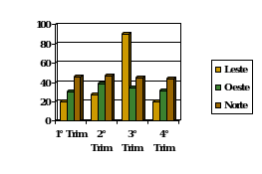
\includegraphics{imagens/img-grafico.png}}
    \caption{Exemplo de apresentação de uma figura no texto (MEREGALI, 2004).}
    \label{fig:grafico}
\end{figure}

\subsection{Citações de fonte nas figuras}

Se  buscada em alguma obra publicada, deve aparecer sempre na descrição da figura, entre parênteses ``(MEREGALI, 2004)''.

Observando que na LISTA DE FIGURAS a fonte não deve aparecer.

\section{Descrição das Tabelas}

Veja exemplo de formatação da Tabela \ref{tab:exemplo-texto} a seguir: a legenda aparece acima da tabela, a descrição deve ser centralizada, no número de identificação \ref{tab:exemplo-texto}, o número 2 corresponde ao capítulo onde se localiza a tabela e o número 1 a ordem da tabela dentro do capítulo, seguido de dois ponto, espaço e  breve descrição, que deve ter a \emph{primeira} letra em maiúsculo.

Observe que as laterais das tabelas são abertas. Isso torna a imagem mais limpa e clara. As tabelas do texto não devem exceder a margem.

\begin{table}[h]
    \caption{Exemplo de apresentação de uma tabela no texto}
    \begin{center}
        \begin{tabular}{ c | c | c }
            \hline
            Manga & Abacaxi & Morango \\
            \hline
            12 & 100.000,00 & 10.000,00 \\
            \hline
            12 & 10.000,00 & 100.000,00 \\
            \hline
        \end{tabular}
    \end{center}
    \legend{Fonte: MEREGALI, 2004. p. 356.}
    \label{tab:exemplo-texto}
\end{table}

\subsection{Citações de fonte nas tabelas}

Se buscada em alguma obra publicada, a citação deve aparecer sempre na descrição da mesma, mas, diferentemente das figuras, a parte abaixo das Tabelas é reservada para a indicação de fontes dos dados, de modo similar a uma nota de rodapé. Contendo autor, ano e página. Veja exemplo acima.

Observando que na LISTA DE TABELAS a fonte não deve aparecer.

\section{Título 2}

xxxxxxxxxx\-xxxxxxxxxx\-xxxxxxxxxx\-xxxxxxxxxx\-xxxxxxxxxx\-xxxxxxxxxx\-xxxxxxxxxx\-xxxxxxxxxx\-xxxxxxxxxx\-xxxxxxxxxx\-xxxxxxxxxx\-xxxxxxxxxx\-xxxxxxxxxx\-xxxxxxxxxx\-xxxxxxxxxx\-xxxxxxxxxx\-xxxxxxxxxx\-xxxxxxxxxx\-xxxxxxxxxx\-xxxxxxxxxx\-xxxxxxxxxx\-xxxxxxxxxx\-xxxxxxxxxx\-xxxxxxxxxx\-xxxxxxxxxx\-xxxxxxxxxx\-xxxxxxxxxx\-xxxxxxxxxx\-xxxxxxxxxx\-xxxxxxxxxx\-xxxxxxxxxx\-xxxxxxxxxx\-xxxxxxxxxx\-xxxxxxxxxx\-xxxxxxxx

\begin{figure}[h]
    \centerline{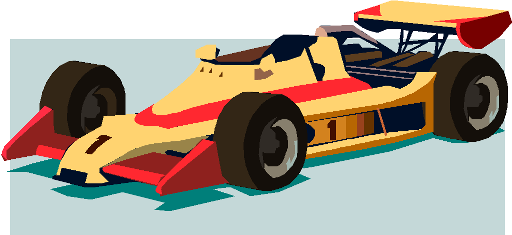
\includegraphics{imagens/img-carro.png}}
    \caption{Outro exemplo de figura}
    \label{fig:carro}
\end{figure}

\subsection{Título 3}

xxxxxxxxxx\-xxxxxxxxxx\-xxxxxxxxxx\-xxxxxxxxxx\-xxxxxxxxxx\-xxxxxxxxxx\-xxxxxxxxxx\-xxxxxxxxxx\-xxxxxxxxxx\-xxxxxxxxxx\-xxxxxxxxxx\-xxxxxxxxxx\-xxxxxxxxxx\-xxxxxxxxxx\-xxxxxxxxxx\-xxxxxxxxxx\-xxxxxxxxxx\-xxxxxxxxxx\-xxxxxxxxxx\-xxxxxxxxxx\-xxxxxxxx

\begin{quote}Citações com mais de 3 linhas devem possuir mais 4 cm de margem, fonte 10 pt, justificada xxxxxxxxxx\-xxxxxxxxxx\-xxxxxxxxxx\-xxxxxxxxxx\-xxxxxxxxx xxxxxxxxxx\-xxxxxxxxxx\-xxxxxxxxxx\-xxxxxxxxxx\-xxxxxxxxxx\-xxxxxxxxxx\-xxxxxxxxxx\-xxxxxxxxxx\-xxxxxxxxxx\-xxxxxxxxxx\-xxxxxxxxxx\-xxxxxxxxxx\-xxxx.\end{quote}

\subsubsection{Subseção}

O nível 4 não aparece no sumário. xxxxxxxxxx\-xxxxxxxxxx\-xxxxxxxxxx\-xxx xxxxxxxxxx\-xxxxxxxxxx\-xxxxxxxxxx\-xxxxxxxxxx\-xxxxxxxxxx\-xxxxxxxxxx\-xxxxxxxxxx\-xxxxxxxxxx\-xxxxxxxxxx\-xxxxxxxxxx\-xxxxxxxxxx\-xxxxxxxxxx\-xxxxxxxxxx\-xxxxxxxxxx\-xxxxxxxxxx\-xxxxxxxxxx\-xxxxxxxxxx\-xxxxxxxxxx\-xxxxxxxxxx\-xxxxxxxxxx\-xxxxxxxxxx\-xxxxxxxxxx\-xxxxxxxxxx\-xxxxxxxxxx\-xxxxxxxxxx\-xxxxxxxxxx\-xxxxxxxxxx\-xxxxxxxxxx\-xxxxxxxxxx\-xxxxxxx.

\subsubsection{Outra subseção}

xxxxxxxxxx\-xxxxxxxxxx\-xxxxxxxxxx\-xxxxxxxxxx\-xxxxxxxxxx\-xxxxxxxxxx\-xxxxxxxxxx\-xxxxxxxxxx\-xxxxxxxxxx\-xxxxxxxxxx\-xxxxxxxxxx\-xxxxxxxxxx\-xxxxxxxxxx\-xxxxxxxxxx\-xxxxxxxxxx\-xxxxxxxxxx\-xxxxxxxxxx\-xxxxxxxxxx\-xxxxxxxxxx\-xxxxxxxxxx\-xxxxxxxxxx\-xxxxxxxxxx\-xxxxxxxxxx\-xxxxxxx.

\subsection{Segundo}

xxxxxxxxxx\-xxxxxxxxxx\-xxxxxxxxxx\-xxxxxxxxxx\-xxxxxxxxxx\-xxxxxxxxxx\-xxxxxxxxxx\-xxxxxxxxxx\-xxxxxxxxxx\-xxxxxxxxxx\-xxxxxxxxxx\-xxxxxxxxxx\-xxxxxxxxxx\-xxxxxxxxxx\-xxxxxxxxxx\-xxxxxxxxxx\-xxxxxxx.

\begin{figure}[h]
    \centerline{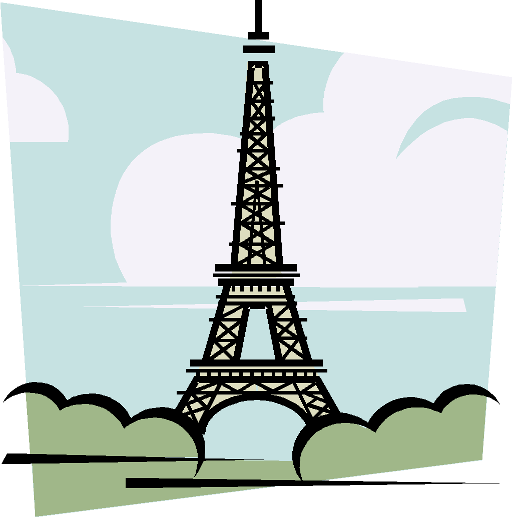
\includegraphics{imagens/img-paris.png}}
    \caption{Terceira figura: Local das férias depois do Trabalho de Conclusão}
    \label{fig:paris}
\end{figure}

\subsection{Terceiro}

xxxxxxxxxx\-xxxxxxxxxx\-xxxxxxxxxx\-xxxxxxxxxx\-xxxxxxxxxx\-xxxxxxxxxx\-xxxxxxxxxx\-xxxxxxxxxx\-xxxxxxxxxx\-xxxxxxxxxx\-xxxxxxxxxx\-xxxxxxxxxx\-xxxxxxxxxx\-xxxxxxxx

\chapter{Citações}

Há duas formas de se fazer uma citação: a \emph{citação indireta ou livre} (também chamada de \emph{paráfrase}) e a \emph{citação direta ou textual}. Pode haver, ainda, a \emph{citação de citação}.

Todas as citações devem trazer a \emph{identificação} de sua autoria.

\section{Citação indireta ou livre (paráfrase)}

Chamamos de citação indireta ou livre (\emph{paráfrase}) aquela citação na qual expressamos o \emph{pensamento de outra pessoa} com \emph{nossas próprias palavras}.

Após fazermos a citação, devemos indicar o nome do autor, \emph{em letras minúsculas}, se estiver no corpo do texto, e com letras \emph{maiúsculas}, se estiver dentro dos parênteses, juntamente com o \emph{ano} da publicação da obra em que se encontra a idéia por nós referida. Não são indicadas páginas já que a idéia pode estar sendo resumida de uma obra inteira, de um capítulo, de diversas partes ou de um conjunto delas.

Desta forma (com o nome no corpo do texto):

Depois de analisar a situação, \citeonline{novoa1993} chegou a afirmar que o brasileiro ainda não está capacitado para escolher seus governantes por causa de sua precária vocação política e da absoluta falta de escolaridade, já que o homem do povo, o zé-povinho, geralmente não sabe sequer em quem votou nas últimas eleições, não sabe sequer quem são seus governantes, não saber sequer quem determina seu próprio meio de sobreviver.

Ou, então, (com o nome nos parênteses):

Depois de analisar a situação, chegou-se a afirmar que o brasileiro ainda não está capacitado para escolher seus governantes por causa de sua precária vocação política e da absoluta falta de escolaridade, já que o homem do povo, o zé-povinho, geralmente não sabe sequer em quem votou nas últimas eleições, não sabe sequer quem são seus governantes, não saber sequer quem determina seu próprio meio de sobreviver \cite{novoa1993}.

No caso de o autor possuir outras obras, elas serão diferenciadas pela data da publicação. Havendo mais de uma obra no mesmo ano, acrescentamos uma letra após a data.

No caso do teatro ou do cinema quem melhor se definiu foi \citeonline{antunes1997a} quando declarou que aqueles espaços haviam sido todos tomados pela geração de 40. Por outro lado, ele próprio se contradisse, mais tarde, \citeonline{antunes1997b}, como já se contradissera noutras ocasiões, ao referir-se às decisões tomadas pelos autores da geração de 50. Isso é uma incongruência com a qual convivemos há muito tempo.

Quando, no transcorrer do texto, em citações indiretas ou livres, se faz menção, seguidas vezes, ao mesmo autor, na mesma obra, não é necessário que se repita a indicação do ano.

\begin{table}[h]
    \caption{ Deve-se escolher somente um tipo de citação para usar durante o texto}
    \begin{center}
        \begin{tabular}{ c | p{0.6\textwidth} }
            \hline
            \multicolumn{2}{ c }{FORMATAÇÃO DAS CITAÇÕES DOS AUTORES DURANTE O TEXTO} \\
            \hline
            \citeonline{novoa1993} & O nome do autor deve ser escrito em letras \emph{minúsculas} quando apresentado no próprio texto \\
            \hline
            \cite[p. 32]{guimaraes1985} & O nome do autor deve ser escrito em letras \emph{maiúsculas} quando apresentado dentro dos parênteses. \\
            \hline
        \end{tabular}
    \end{center}
    \legend{Fonte: \citeauthor{meregali2004}, \citeyear{meregali2004}, p. 356.}
    \label{tab:tipos-citacao}
\end{table}

\section{Citação direta ou textual (transcrição)}

São chamadas de citações diretas ou textuais aquelas em que se transcrevem \emph{exatamente as palavras do autor citado}. As citações diretas ou textuais podem ser \emph{breves} ou \emph{longas}.

São consideradas \emph{breves} aquelas cuja extensão não ultrapassa \emph{três linhas}. Essas citações devem \emph{integrar o texto} e devem vir \emph{entre aspas}. \emph{O tamanho} da \emph{fonte} (letra) da citação breve \emph{permanece} o mesmo do corpo do texto (\emph{pitch 12}).

Vimos que, para nosso esclarecimento, precisamos seguir os preceitos encontrados, já que \citeauthoronline{guimaraes1985} estabelece: ``A valorização da palavra pela palavra encarna o objetivo precípuo do texto literário'' (\citeyear{guimaraes1985}, p. 32) e, se isso não ficar bem esclarecido, nosso trabalho será seriamente prejudicado.

Ou assim:

Vimos que, para nosso esclarecimento, precisamos seguir os preceitos encontrados, já que ficou estabelecido que ``a valorização da palavra pela palavra encarna o objetivo precípuo do texto literário'' \cite[p. 32]{guimaraes1985} e, se isso não ficar bem esclarecido, nosso trabalho será seriamente prejudicado.

As citações com mais de três linhas são chamadas de \emph{longas} e devem receber um destaque especial com recuo (reentrada) de \emph{4cm} ou \emph{dezesseis toques}, da margem, mais \emph{cinco} toques para o início do parágrafo.

As citações longas, por já terem o destaque do recuo (reentrada), \emph{não deverão ter aspas} e o tamanho da fonte (letra) deve ser \emph{menor} que o do texto: \emph{pitch 10}.

A distância entre as linhas do corpo da citação deve ser de um espaço \emph{simples}. Entre o texto da citação e o restante do trabalho, deve-se deixar \emph{dois espaços duplos}, antes e depois.

Há uma certa dificuldade quanto ao reconhecimento de \emph{O, A, OS, AS} como pronomes demonstrativos, mas essa dúvida é muito bem dirimida por \citeyear{fernandes1994}:

\begin{quote}Os pronomes O, A, OS e AS passam a ser pronomes demonstrativos sempre que numa frase puderem ser substituídos, sem alterar a estrutura dessa frase, respectivamente, por ISTO, ISSO, AQUILO, AQUELE, AQUELES, AQUELA, AQUELAS (\citeyear{fernandes1994}, p. 19.).\end{quote}

Havendo \emph{supressão} de trechos \emph{dentro do texto} citado, faz-se a indicação com reticências entre colchetes [\ldots]:

``Na comunicação diária, aquela comunicação que utilizamos no dia-a-dia, junto de nossos familiares e amigos, por exemplo, além da referencialidade da linguagem [\ldots] há pinceladas de função conativa'' \cite[p. 37]{chalhub1991}.

No \emph{início} ou no \emph{fim} da citação, as reticências são usadas apenas quando o trecho citado \emph{não é uma sentença completa}. Entende-se por sentença completa aquela que o autor elaborou, com todos os seus elementos, isto é, uma sentença que contenha sujeito, predicado e seus complementos gramaticais exigidos. Caso contrário, \emph{se a sentença for completa}, no início ou no termino de citação, \emph{não se deve fazer} o uso das reticências. \emph{É óbvio} que se trata de parte de um todo, que se retirou um trecho, portanto, não há necessidade de se indicar com as reticências.

Encerrava seu discurso nomeando os que figurariam somente nos exercício gerais, citando palavras de ordem, dentre as quais pudemos entender:

``\ldots muitas mortes, desaparecimentos e desolação haverão de varrer este pais de norte a sul, de lesta a oeste e nada restará para a posteridade que sentirá a falta de um elo'' \cite{morgado1967}.

Mais adiante, aquilo que mais chocou a todos quanto o ouviam:

``Arrasem com tudo, queimem tudo, ponham tudo abaixo, destruam com tudo, não poupem ninguém, nem crianças, nem mulheres, nem velhos\ldots'' \cite{morgado1967}.

Se a citação for usada para completar uma sentença do autor do Trabalho, esta terminará em vírgula e aquela iniciará \emph{sem a entrada de parágrafo} e \emph{com letra minúscula}.

A secretária ameaçou, dizendo que, ``da próxima vez, a máquina ficará sem as peças de reposição, se ele não chegar e disser o que precisa ser dito, uma vez que não estou aqui para servir de adivinha para seus caprichos desencontrados e sem nexo.'' \cite[p. 34]{marques1982}.

Caso o texto do autor do Trabalho seja uma \emph{continuação} da citação, esta \emph{terminará por vírgula} e o texto reiniciado \emph{sem entrada de parágrafo e com letra minúscula}.

 Os gramáticos são claros quando assumem uma posição quanto ao emprego do pronome oblíquo no início de oração. \citeonline[p. 419]{cegalla1991} diz claramente que: \begin{quote}Iniciar a frase com o pronome átono só é lícito na conversação familiar, despreocupada, ou na língua escrita, quando se deseja reproduzir a fala dos personagens, porém nós sabemos que na prática não é bem assim que acontece - as normas, rigorosamente, são esquecidas por quase todos os usuários do idioma falado, principalmente nas ocasiões informais.\end{quote}

Quando houver uma citação \emph{dentro de outra citação}, as aspas da segunda transformam-se em aspas simples (` e ') (apóstrofo: Não confundir a palavra \emph{apóstrofo} que é o sinal (` e '), com \emph{apóstrofe} que é uma figura de linguagem que consiste na interpelação ou invocação do leitor, ouvinte ou outra pessoa no decorrer de um texto). Quando dentro da citação transcrita houver aspas, estas também são mudadas para aspas simples.

Se for feita alguma \emph{interpelação}, \emph{acréscimo} ou \emph{comentário} durante a citação, deve-se fazê-lo \emph{entre colchetes} [ ]:

Também chamado de corpo do trabalho, [o desenvolvimento] tem por finalidade expor, demonstrar e fundamentar a explicitação do assunto a ser abordado. É normalmente dividido em seções ou capítulos, que variam de acordo com a natureza do assunto. \cite[p. 17]{garcia2000}.

Se algum \emph{destaque} (grifo, negrito, itálico ou sublinhado) for dado, deve-se indicá-lo com a expressão \emph{grifo nosso}, entre colchetes:

A primeira citação de uma obra deve ter sua referência bibliográfica completa. As subseqüentes citações da mesma obra \emph{podem ser referendadas de forma abreviada}, desde que não haja referências intercaladas de outras obras do mesmo autor (NBR 6023-2000) [\emph{grifo nosso}].

Caso o texto citado traga algum tipo de destaque dado pelo autor do trecho, devemos usar a expressão \emph{grifo do autor, entre colchetes}.

A verdadeira felicidade é encontrada nos pequenos detalhes que vão se somando \emph{dia após dia} de convivência com o ser amado \cite[p. 12]{guerrero2000} [\emph{grifo do autor}].

Quando o texto citado for composto por informações orais obtidas em aulas, palestras, debates, comunicações, etc. deve-se, entre parênteses, colocar a observação \emph{informação oral}, mencionando-se os dados disponíveis em nota de rodapé:

Eichenberg constatou que, na costa do Rio Grande do Sul, especialmente no litoral norte, há a presença abundante de conformes fecais, especialmente nos meses do verão (informação oral). Essa presença tem causado graves transtornos a todos os veranistas.

Se for o caso de se fazer menção a algo contido em \emph{polígrafos}, \emph{apostilas} ou quaisquer materiais avulsos, faz-se a indicação do nome do autor, quando for possível sua identificação, acrescentando-se a observação \emph{`polígrafo'}, \emph{`material de propaganda'}, \emph{`panfleto'}, etc. Procede-se da mesma forma com relação à data. Indica-se, se houver, caso contrário, registra-se s.d. (sem data).

\begin{table}[h]
    \caption{Observação quanto às aspas}
    \begin{center}
        \begin{tabular}{ p{\textwidth} }
            \hline
            As ações longas (mais de três linhas) \emph{não recebem aspas} letra é menor (tamanho 10) do que a do texto (tamanho 12). \\
            \hline
             \\
            \hline
        \end{tabular}
    \end{center}
    \legend{Fonte: \citeauthor{furaste2000}, \citeyear{furaste2000}, p. 100.}
    \label{tab:tipos-citacao-longa}
\end{table}

\section{Citação de citação}

Se, num Trabalho, for feita uma citação de alguma passagem \emph{já citada em outra obra}, a autoria deve ser referenciada pelo \emph{sobrenome do autor original} seguido da palavra latina \emph{apud} (que significa \emph{segundo}, \emph{conforme}, \emph{de acordo com}) \emph{e o sobrenome do autor da obra consultada}. Dessa última, faz-se a referência completa (NBR6O23).

``O sistema consiste em colocar o recém-nascido no berço, ao lado da mãe, logo após o parto ou algumas horas depois, durante a estada de ambos na maternidade'' \apud[p. 79]{harunari}{guaragna1992}.

Temos aí palavras de Harunari que foram citadas por Guaranga e que estão sendo utilizadas, agora, no meu trabalho.

\emph{Fonte}: FURASTÉ, Pedro Augusto. Normas Técnicas para o Trabalho Científico: explicitação das normas da ABNT. Porto Alegre: [s.n.], 2002. p. 49-56.

\input{conteudo/resultados-discussoes.tex}
\chapter{Conclusão}

Apresentar conclusão do trabalho xxxxxxxxxx\-xxxxxxxxxx\-xxxxxxxxxx\-xxxxx xxxxxxxxxx\-xxxxxxxxxx\-xxxxxxxxxx\-xxxxxxxxxx\-xxxxxxxxxx\-xxxxxxxxxx\-xxxxxxxxxx xxxxxxxxxx\-xxxxxxxxxx\-xxxxxxxxxx\-xxxxxxxxxx\-xxxxxxxxxx\-xxxxxxxxxx\-xxxxxxxxxx\-xxxxxxxxxx\-xxxxxxxxxx\-xxxxxxxxxx\-xxxxxxxxxx\-xxxxxxxxxx\-xxxxxxxxxx\-xxxxxxxxxx\-xxxxxxxxxx\-xxxxxxxxxx\-xxxxxxxxxx\-xxxxxxxxxx\-xxxxxxxxxx\-xxxxxxxxxx\-xxxxxxxxxx\-xxxxxxxxxx\-xxxxxxxxxx\-xxxxxxxxxx\-xxxxxxxxxx\-xxxxxxxxxx\-xxxxxxxxxx\-xxxxxxxxxx

\bibliographystyle{abntex2-alf}
\bibliography{biblio}
\end{document}
